\documentclass{llncs}
\pagestyle{plain}
\usepackage[hide]{ed}
\usepackage[utf8]{inputenc}
\usepackage{xspace}
\usepackage{amssymb}
\usepackage{wrapfig}
\usepackage[style=alphabetic,backend=bibtex,isbn=false]{biblatex}
\addbibresource{../../lib/kbibs/kwarcpubs.bib}
\addbibresource{../../lib/kbibs/extpubs.bib}
\addbibresource{../../lib/kbibs/kwarccrossrefs.bib}
\addbibresource{../../lib/kbibs/extcrossrefs.bib}
\addbibresource{rest.bib}% add bibs here!
\renewbibmacro*{event+venue+date}{}
\renewbibmacro*{doi+eprint+url}{%
  \iftoggle{bbx:doi}
    {\printfield{doi}\iffieldundef{doi}{}{\clearfield{url}}}
    {}%
  \newunit\newblock
  \iftoggle{bbx:eprint}
    {\usebibmacro{eprint}}
    {}%
  \newunit\newblock
  \iftoggle{bbx:url}
    {\usebibmacro{url+urldate}}
    {}}

% identifiers and URIs
\providecommand{\identifier}[1]{%
  \StrSubstitute{#1}{\_}{_}[\identifiertmp]
  \expandafter\path\expandafter{\identifiertmp}%
}
\let\uri\identifier

% TIKZ
\usepackage{tikz}
\def\thmo#1#2{\mathsf{#1}\colon\kern-.15em{#2}}% for theories
\usetikzlibrary{shapes,arrows,fit,shadows}

% Abbreviations
\providecommand{\mmt}{MMT}
\providecommand{\omdocmmt}{OMDoc/MMT}
\providecommand{\lmfdb}{LMFDB}

% code snippets
\usepackage{listings}
\lstdefinelanguage{qmt}{
    basicstyle=\footnotesize\ttfamily,
    showstringspaces=false,
    frame=single, 
    mathescape, 
    columns=fullflexible,
    breaklines=true
}
\providecommand{\inlinecode}[1]{{\lstinline[language=qmt]|#1|}}

\def\meta#1{\ensuremath{\langle\kern-.25em\langle}#1\ensuremath{\rangle\kern-.2em\rangle}}

% More abbreviatons for diagrams and things
\def\plaintt#1{\ifmmode\mathrm{\texttt{#1}}\else\texttt{#1}\fi}
\def\typett{\plaintt{type}}
\def\codectt{\plaintt{codec}}


\usepackage{hyperref}
\title{REGULAR-T1: Virtual Theories -- A Uniform Interface to Mathematical Knowledge Bases}
\author{
Tom Wiesing\inst{1}
Michael Kohlhase\inst{1} 
Florian Rabe\inst{2} 
}

\institute{
   FAU Erlangen-N\"urnberg
   \and Jacobs University Bremen
%   \and Universit\'e Paris-Sud
}
\begin{document}
\maketitle
\begin{abstract}
  There are various mathematical knowledge collections and information systems
  available. They range from completely informal ones like Wikipedia or the Cornell arXiv,
  zbMath, and MathSciNet via mathematical object databases like the GAP group libraries,
  the Online Encyclopedia of Integer sequences (OEIS), and the L-functions and Modular
  Forms Database (LMFDB) to theorem prover libraires like those of Mizar, Coq, PVS, and
  the HOL systems.\ednote{continue}
\end{abstract}

\ednote{Target Size: 15 pages}

In this report we present a prototypical integration of the Jupyter notebooks into the MathHub.info portal for active mathematical documents and a versioned hosting system for flexiformal mathematics.
MathHub.info offers a rich interface for reading, writing, and interacting with mathematical documents and knowledge. Jupyter offers a uniform interface to the computation facilities of the OpenDreamKit VRE toolkit in the form of a read-eval-print loop (REPL).

A mathematical Virtual Research Environment (VRE) needs both kinds of interface functionality: mathematical documents have been very successful for presenting mathematical knowledge, and while there have been efforts to make them modular and interactive they predominantly remain in the mode of archiving and transporting knowledge in Mathematics.
Notebook interfaces also use the document metaphor at the surface; however the REPL interaction
tends to take structural precedence, leading to documents consisting of a sequence of computational cells within which the mathematical discourse is interspersed in the form of ``rich comments''.

A ``literate computing'' version of notebooks which gives mathematical discourse structural precedence is possible in principle, but has not been supported consistently at the system level.\ednote{MK: put the following sentence somewhere: A ``literate programming'' version of notebooks which gives mathematical discourse structural precedence is possible in principle, but has not been supported consistently at the system level.}
This tension and trade-off has been explored in OpenDreamKit Deliverable D4.2~\cite{ODK-D4.2}, and the concept of in-document computation in OpenDreamKit Deliverable D4.9~\cite{ODK-D4.9}.
In both cases, the integration was incomplete, since it lacked a full integration of the
underlying knowledge/computation services.

Generally, the integration of MathHub and Jupyter consists of two parts:
\begin{inparaenum}[\em a\rm )]
\item the integration of the user interfaces (as reported previously) and
\item the integration of the knowledge/computation management services.
\end{inparaenum}
Here we report on progress in both; recall that MMT is the knowledge management service behind MathHub (and more generally for the Math-in-the-Middle based system integration; see OpenDreamKit Deliverable D6.5~\cite{ODK-D6.5}).
%
For the service integration we present an MMT kernel for Jupyter.
%
\ednote{specify what Jupyter widgets are; NT: you may want to reuse some of the language of the D4.16 report, around l21 of https://github.com/OpenDreamKit/OpenDreamKit/blob/master/WP4/D4.16/report.tex}
%
Reciprocally, for the user interface integration, we show how the Jupyter widgets can be deeply integrated within the MMT knowledge management facilities to give semantics-aware interaction facilities, extending the front-end capabilities of MathHub/Jupyter Notebooks by semantic widgets driven by the MMT in-document knowledge management services.

We show and evaluate the integration on two case studies: in-document computing facilities in active documents and a knowledge-based specification dialog for modeling and simulation. 

This report is structured as follows. In Section~\ref{sec:mmt-jp} we report on the MathHub/Jupyter integration at the system level: a Jupyter server as part of the MathHub system and a MMT kernel for Jupyter. Section~\ref{sec:nb-mh} presents the integration of Jupyter Notebooks as active documents in the (new) MathHub front-end, and Section~\ref{sec:mitm-nb} presents the two case studies. Section~\ref{sec:concl} concludes the report and discusses future work.

\ednote{this paragraph seems a bit out of place after the description of the structure of the document}
The goal of this report\ednote{of this deliverable?} is to integrate Jupyter notebooks into MathHub
and make them compatible with MMT, in a way that we can conveniently use 
MMT syntax in these notebooks and also a little bit of extra functionality
like e.g. the Jupyter widgets. The first step is setting up a Jupyter server,
which currently runs on \url{http://juypter.mathhub.info}. \ednote{KA: maybe show picture of it?}
For this server, we have developed a custom kernel, that forwards the input 
entered into the Jupyter notebook to the MMT backend. This then processes 
said input and sends the response back to the Jupyter frontend via the kernel.
We will cover the implementation of the Jupyter kernel and the MMT-backend,
later in this report.


\paragraph{Acknowledgements} The authors gratefully acknowledge the support of the Jupyter team and in particular the advice of Benjamin Ragan-Kelly. Also, the input of Theresa Pollinger and her work on the MoSIS system~\cite{PolKohKoe:kacse18} has shaped our perception of the integration reported here. 

%%% Local Variables:
%%% mode: latex
%%% mode: visual-line
%%% fill-column: 5000
%%% TeX-master: "report"
%%% End:

\section{Example: The API and Structure of LMFDB}\label{sec:sota}

The ``L-functions and Modular Forms Database'' (\lmfdb~\cite{lmfdb}) is a Python web
application with a MongoDB backend.  The project contains several thousand L-Functions and
curves along with their properties. We use this as an example of a Virtual Theory.  Before
we go into this in more detail, we first have a closer look at the structure and existing
APIs to communicate with it.

\subsection{The Structure of LMFDB}\label{sec:sota:struct}

\lmfdb has several sub-databases -- each of which contains different kinds of objects.
These databases include e.g. a database of elliptic curves or a database of transitive
groups.  Within each database, each curve is stored as a single JSON record with common
keys, Figure~\ref{fig:lmfdbexample} shows one: each property of this JSON object corresponds to a property of the underlying mathematical object. 
For example, the \identifier{degree} property -- here $1$ -- of the JSON objects corresponds to the degree of the underlying elliptic curve. 


\begin{figure}[ht]\centering
      \begin{lstlisting}[language=json]
{
    "degree": 1,
    "non-maximal_primes": [5],
    "torsion_structure": ["5"],
    "ainvs": ["0","-1","1","-10","-20"],
    "x-coordinates_of_integral_points": "[5,16]",
    "real_period": 1.26920930427955,
    "min_quad_twist": {"disc": 1,"label": "11a1"},
    "sha_an": 1.0,
    "conductor": 11,
    "iwp0": 7,
    "2adic_gens": [],
    "torsion_primes": [5],
    "signD": -1,
    "tamagawa_product": 5,
    "isogeny_matrix": [[1,5,25],[5,1,5],[25,5,1]],
    "non-surjective_primes": [5],
    "lmfdb_label": "11.a2",
    "2adic_index": 1,
    "equation": "\\( y^2 + y = x^{3} -  x^{2} - 10 x - 20  \\)",
    "label": "11a1",
    "regulator": 1.0,
    "anlist": [0,1,-2,-1,2,1,2,-2,0,-2,-2,1,-2,4,4,-1,-4,-2,4,0,2],
    "iso": "11a",
    "_id": "ObjectId('4f71d4304d47869291435e6e')"
}
      \end{lstlisting}\vspace*{-1.5em}
  \caption[An elliptic curve from \lmfdb]{
    An elliptic curve, as found within \lmfdb. 
    Some key-value pairs are omitted for readability. 
  }
  \label{fig:lmfdbexample}
\end{figure}

Other properties are more complex.
Whereas the value of the \identifier{degree} property is a simple integer, the value of
the \identifier{isogeny\_matrix} property is a list of lists, which represents a matrix. 
This can become even more technical. 
For example the \identifier{x-coordinates\_of\_integral\_points} field, \lmfdb represents
a list of integers as a list of strings as the integers can exceed the range of MongoDB system
integers.  This already shows that it is non-trivial to get from a MongoDB encoding of an elliptic
curve in \lmfdb to the representation of a mathematical object. 


\subsection{An API for  \lmfdb Objects}\label{sec:sota:api}

As \lmfdb is is a mathematical knowledge base, one important use case is to find elliptic
curves subject to specific criteria. As a very simple example, suppose a mathematician
wants to find all Abelian elliptic curves.  How can this be achieved using the \lmfdb API
at \url{http://www.lmfdb.org/api/transitivegroups/groups/}\ednote{Proper citation}.

\begin{figure}[ht]\centering
  \includegraphics[width=\textwidth]{APIScreenshot.png}
  \caption[The Web-Interface for the \lmfdb API. ]{
    The Web-Interface for the \lmfdb API. 
  }
  \label{fig:apiscreenshot}
\end{figure}

This API has two basic modes. The first allows allows to make searches using the
web-browser.  Users can manually enter a query, and see a list of results displayed.  A
screenshot of this interface is shown in Figure~\ref{fig:apiscreenshot}.  In the other
mode queries can be given as JSON directly.  This can be used in automated scenarios.

In both of these mods queries must be formulated in terms of the underlying MongoDB
schema. For example, to search for all abelian elliptic curves, we must know that the
\identifier{ab} key corresponds to the commutativity property, has Boolean values, and
that MongoDB encodes \inlinecode{true} as \inlinecode{1}, and \inlinecode{false} as
\inlinecode{0} in this \lmfdb sub-database. This information can then be used to make a
request to \url{http://www.lmfdb.org/api/transitivegroups/groups/?ab=1}. This finds all
Abelian, transitive groups.

In this example, each of the steps are relatively straightforward. 
In a general setting, e.g. when searching for all elliptic curves with a specific isogeny
matrix, this not only requires a good familiarity with the mathematical background but
also with the system internals of the particular \lmfdb sub-database; a skillset commonly
found in neither research programmers nor average mathematicians.   

To summarize: while \lmfdb offers a programmable API for accessing its contents, the
content API is at the MongoDB level, and not the level of mathematical objects. Our
Diagnosis is that \lmfdb -- and most other mathematical knowledge databases -- suffer from
a double impedance mismatch problem.
\begin{compactenum}[\bf {I}1]
\item \emph{human/computer impedance mismatch}: Humans have problems interacting with
  \lmfdb, since they must speak the system language instead \lmfdb speaking mathematics
\item \emph{computer/computer impedance mismatch}: mathematical computer systems cannot
  interoperate, since their system languages differ.
\end{compactenum}
In the MitM approach we have presented in Section~\ref{sec:mmtmitm}, we can solve both
problems at the same time by lifting the communication to the level of \ommt-encoded MitM
objects, which both MitM-compatible software systems and humans speak -- this is the
central assumption of the MitM approach.
%%% Local Variables:
%%% mode: latex
%%% TeX-master: "paper"
%%% End:

%  LocalWords:  sec:sota lmfdb lmfdb lstlisting json ainvs iwp0 2adic_gens isogeny_matrix
%  LocalWords:  tamagawa_product 2adic_index anlist 4f71d4304d47869291435e6e vspace emph
%  LocalWords:  fig:lmfdbexample isogeny includegraphics textwidth fig:apiscreenshot
%  LocalWords:  centering summarize sec:mmtmitm ommt-encoded

\section{Virtual Research Environments for Mathematics: the Math-in-the-Middle
  Approach}\label{sec:mmtmitm}

The work reported in this paper originates from in the EU-funded \textsf{OpenDreamKit}
\cite{OpenDreamKit:on} project that aims to create virtual research environments (VRE)
enabling mathematicians to make efficient use of existing open-source mathematical
knowledge systems.  These systems include computer algebra systems like SageMath and GAP
as well as mathematical data bases such as the \lmfdb, which must be made interoperable
for integration into a VRE. In the \textsf{OpenDreamKit} project we have developed the
Math-in-the-Middle (MitM) approach, which posits a central ontology of mathematical
knowledge, which acts as a pivot point for interoperability; see~\cite{DehKohKon:iop16}
for a description of the approach and \cite{KohMuePfe:kbimss17} for a technical refinement
and large-scale interoperability case study. 

\begin{wrapfigure}l{0.3\textwidth}%\vspace*{-2em}
    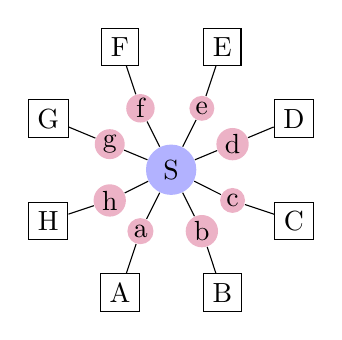
\begin{tikzpicture}[xscale=1.3,yscale=1.3]\normalsize
      \tikzstyle{withshadow}=[draw,drop shadow={opacity=.5},fill=white]
      \tikzstyle{system}=[draw]
      \tikzstyle{standard}=[circle,fill=blue!30]
      \tikzstyle{interface}=[circle,fill=purple!30,inner sep = 1pt,]
      \node[system] (a) at (0,.3) {A};
      \node[system] (b) at (1,.3) {B};
      \node[system] (c) at (1.7,1) {C};
      \node[system] (d) at (1.7,2) {D};
      \node[system] (e) at (1,2.7) {E};
      \node[system] (f) at (0,2.7) {F};
      \node[system] (g) at (-.7,2) {G};
      \node[system] (h) at (-.7,1) {H};
      \node[standard] (m) at (.5,1.5) {S};
      \node[interface] (ia) at (0.2,.9) {a};
      \node[interface] (ib) at (.8,.9) {b};
      \node[interface] (ic) at (1.1,1.2) {c};
      \node[interface] (id) at (1.1,1.75) {d};
      \node[interface] (ie) at (.8,2.1) {e};
      \node[interface] (if) at (0.2,2.1) {f};
      \node[interface] (ig) at (-.1,1.75) {g};
      \node[interface] (ih) at (-.1,1.2) {h};
      \draw (m) -- (ia) -- (a);
      \draw (m) -- (ib) -- (b);
      \draw (m) -- (ic) -- (c);
      \draw (m) -- (id) -- (d);
      \draw (m) -- (ie) -- (e);
      \draw (m) -- (if) -- (f);
      \draw (m) -- (ig) -- (g);
      \draw (m) -- (ih) -- (h);
      \end{tikzpicture}
  \caption{The MiTM Approach to Connecting Systems.}\label{fig:mitmconnect}\vspace*{-1em}
\end{wrapfigure}
The MitM ontology in the center of Figure~\ref{fig:mitmconnect} models the true,
underlying mathematical semantics in \ommt and allows translation between this centrally
formalized knowledge and the systems on the boundary via views and alignments.
This mathematical knowledge is modeled using the well-established theory graph paradigm
and is stored inside our \ommt-based MathHub system~\cite{MathHub:on}. 

The knowledge in the mathematical software systems -- denoted by square boxes in
Figure~\ref{fig:mitmconnect} -- also modeled via \ommt theory graphs the \textbf{API
  theories} -- the corresponding red circles; these are generated from the
knowledge bases in the systems by a custom process. The API theories allow us to implement
translation with the help of \ommt views and alignments between the ontology -- the
Math-In-The-Middle -- and each of the systems and use these translations for transporting
computational tasks between the systems. 

The realization of the MitM approach crucially depends on the information architecture of
the \ommt language~\cite{Kohlhase:OMDoc1.2,RabKoh:WSMSML13} and its implementation in the
\mmt system~\cite{Rabe:MAGMS13,uniformal:on}.

In \ommt knowledge is organized in \textbf{theories}, which contain information about
mathematical concepts and objects in the form of \textbf{declarations}. Theories are
organized into an ``object-oriented'' inheritance structure via \textbf{inclusions} and
\textbf{structures} (for controlled multiple inheritance), which is augmented via
truth-preserving mappings between theories called \textbf{views}, which allow to relate
concepts of pre-existing theories and transport theorems between these. Inclusions,
structures, and views impose a graph structure on the represented mathematical knowledge,
called a \textbf{theory graph}. 

We observe that even very large mathematical knowledge spaces about abstract mathematical
domains can be represented by small, but densely connected, theory graphs, if we make all
inherited material explicit in a process called \textbf{flattening}. The \ommt language
provides systematic names (\mmt URIs) for all objects, properties, and relations in the
induced knowledge space, and given the represented theory graph, the \mmt system can
compute them on demand. 

Generally, knowledge in a knowledge space given by a theory graph loaded by the \mmt system can be accessed by either giving it's \mmt URI, or by uniquely describing it via a set of conditions. 
To achieve the latter, \mmt has a Query Language called QMT~\cite{Rabe:qlfml12}, which allows even complex conditions to be specified. 
Currently, the \mmt system loads the theory graph into main memory at startup and interleaves incremental flattening and query evaluation operations on the \mmt data structures until the result has been produced. 

In \cite{KohMuePfe:kbimss17} we show that the MitM approach, its \ommt-based realization,
and distribution via the SCSCP protocol are sufficient for distributed, federated computation
between multiple computer algebra systems (Sage, GAP, and Singular), and that the MitM
ontology of abstract group theory can be represented in \ommt efficiently. This setup is
effective because
\begin{compactitem}
\item the knowledge spaces behind abstract and computational mathematics can be represented in theory graphs very space-efficiently: The compression factors between a knowledge space and its theory graph -- we call it the \textbf{TG factor} -- exceeds two orders of magnitude even for small domains.
\item only small parts of the knowledge space are traversed for a given computation. 
\end{compactitem}

But the \textsf{OpenDreamKit} VRE must also include mathematical data sources like the \lmfdb or the OEIS, which contain millions of mathematical objects. For such knowledge sources, the classical \mmt system is not yet suitable:
\begin{compactitem}
\item the knowledge space corresponding to the data base content cannot be compressed by ``general mathematical principles'' like inheritance. 
Indeed, redundant information is already largely eliminated by the data base schema and the ``business logic'' of the information system it feeds.
\item typically large parts of the knowledge space need to be traversed to obtain the intended results to queries.
\end{compactitem}
Therefore, we extend the concept of \ommt theories -- which carry the implicit assumption of containing only a small number of declarations (see~\cite{FaGu:lt92} for a discussion) -- to \textbf{virtual theories}, which can have an unlimited (possibly infinite) number of declarations. 
To contrast the intended uses we will call the classical \ommt theories \textbf{concrete theories}.  
In practice, a virtual theory is represented by concrete approximations: \ommt works with a concrete theory, whose size changes dynamically as a suitable backend infrastructure generates declarations on demand.


%%% Local Variables:
%%% mode: latex
%%% TeX-master: "paper"
%%% End:

%  LocalWords:  omdocmmt fig:classicalconnect fig:mitmconnect OpenDreamKit:on lmfdb lmfdb 1.3,yscale 30,inner compactitem
%  LocalWords:  ODKproposal:on DehKohKon:iop16 sagemath oeis fig:mitmontology colored ig
%  LocalWords:  mathrm mathrm sec:mmtmitm ommt mechanized uniformal:on organized textit
%  LocalWords:  BusCapCar:oms04 MathHub:on Iancu:phd SMGloM:on formalizations wrapfigure
%  LocalWords:  PVSlibraries:on mizar:online textwidth tikzpicture xscale 1.3,yscale
%  LocalWords:  tikzstyle withshadow draw,drop circle,fill 30,inner formalized vspace
%  LocalWords:  MACIS17-interop KohMuePfe:kbimss17 1.3,yscale 30,inner fit:mitmconnect
%  LocalWords:  textbf realization RabKoh:WSMSML13 Rabe:MAGMS13,uniformal:on Rabe:qlfml12
%  LocalWords:  FaGu:lt92

% !TEX root = ../thesis.tex
\section{\lmfdb as a Set of Virtual Theories}\label{sec:vt}

The mathematical software systems to be integrated via the MitM approach have so far been computation-oriented, e.g. computer algebra systems.
Their API CDs typically declare types and functions on these types (the latter including constants seen as nullary functions).
Even though database systems differ drastically from these in many respects, they are very similar at the MitM level: a database like \lmfdb defines
\begin{compactitem}
 \item some types: each table's schema is essentially one type definition,
 \item many constants: each entry of each table is one constant of the corresponding type.
\end{compactitem}
Thus, we can apply essentially the same approach.
In particular, the API CDs must contain definitions of the database schemas. 

From a system perspective, virtual theories behave just like concrete theories, but without the assumption of loading all declarations from a file on disk at system startup.
Instead, virtual theories load declarations in a lazy fashion when they are needed. 
Concrete theories are stored as XML files; i.e. we use the file system as a backend for the \mmt system. 
As most of the knowledge sources we want to embed into \ommt as virtual theories use data-bases as back-ends and provide low-level database APIs we have extended the \mmt backends for this as well.
Apart from standard software engineering tasks, there were three conceptual problems to be solved in this extension/implementation:
\begin{compactenum}[\bf P1]
\item How to match the database tables into \ommt theories and declarations. 
\item How to lift data in \textbf{physical representation} -- i.e. as records of the
  underlying database to \ommt terms -- i.e. data in \textbf{semantic representation}.
\item And how to translate QMT queries from semantic to physical representation -- i.e. so
  that they can be executed directly on the data base without loading bulk data into the
  \mmt process.
\end{compactenum}

\begin{figure}[ht]\centering
    \begingroup
    \pgfdeclarelayer{background}
    \pgfdeclarelayer{foreground}
    \pgfsetlayers{background,foreground}
    
    \resizebox{\textwidth}{0.75\textwidth}{
      \begin{tikzpicture}[xscale=4,yscale=2.2]\footnotesize
        \begin{pgfonlayer}{foreground}
          \tikzstyle{human}    = [red,dashed,thick]
          \tikzstyle{withshadow}  = [draw,drop shadow={opacity=.5},fill=white]
          \tikzstyle{interface}   = [fill=blue!30]
          \tikzstyle{database}    = [cylinder,cylinder uses custom fill,
            cylinder body fill=yellow!50,cylinder end fill=yellow!50,
            shape border rotate=90,
            aspect=0.25,draw]
          
          % Ontology layer
          \node[thy] (numbers) at (0,1) {
            \begin{tabular}{lll}
              \multicolumn{3}{l}{\textsf{Numbers}}\\\hline\hline
              $\mathbb{Z}^{+}$        & : & \typett\\
              $\mathbb{Z}$            & : & \typett\\\hline
              \multicolumn{3}{l}{$\mathbb{Z}^{+} \subset \mathbb{Z}$}
            \end{tabular}
          };

          \node[thy] (matrices) at (1.5,1) {
            \begin{tabular}{lll}
              \multicolumn{3}{l}{\textsf{Matrices}}\\\hline\hline
              \plaintt{matrix} & : & $\typett \rightarrow \mathbb{Z}^{+}\rightarrow \mathbb{Z}^{+} \rightarrow \typett$
            \end{tabular}
          };

          \node[thy] (codecs) at (0.75,0) {
            \begin{tabular}{lll}
              \multicolumn{3}{l}{\textsf{Codecs}}\\\hline\hline
              \codectt                  & : & $\typett \rightarrow \typett$\\\hline
              \plaintt{standardInt}     & : & $\codectt\; \mathbb{Z}$\\
              \plaintt{standardMatrix}  & : & $\left\{T, n, m\right\} \codectt\; T \rightarrow \codectt\; \plaintt{matrix}(n, m, T)$\\
            \end{tabular}
          };

          \draw[include] (numbers) -- (matrices);
          \draw[include] (matrices) -- (codecs);
          
          \begin{pgfonlayer}{background}
            \node[draw=none,fill=green!30,rounded corners=1cm,fit=(numbers) (matrices) (codecs),inner sep=10pt] {};
          \end{pgfonlayer}
        
          % Model Layer
          \node[thy,fill=purple!30] (ec) at (2.25,-1.20) {
            \begin{tabular}{lll}
              \multicolumn{3}{l}{\textsf{Elliptic Curve}}\\\hline\hline
              \plaintt{ec}            & : & \typett\\\hline
              \plaintt{from\_record}  & : & $\plaintt{record} \rightarrow \plaintt{ec}$ \\\hline
              \plaintt{curveDegree}   & : & $\plaintt{ec} \rightarrow \mathbb{Z}$ \\
              \plaintt{isogenyMatrix} & : & $\plaintt{ec} \rightarrow \plaintt{matrix}(3, 3, \mathbb{Z})$ 
            \end{tabular}
          };

          \node[thy,interface] (ecschema) at (2.0,-2.5) {
            \begin{tabular}{lll}
              \multicolumn{3}{l}{\textsf{Elliptic Curve Schema}}\\\hline\hline
              $\plaintt{degree}$            & \uri{?implements}  & \plaintt{curveDegree} \\
                                            & \uri{?codec}       & \plaintt{StandardInt} \\\hline
              $\plaintt{isogeny\_matrix}$   & \uri{?implements}  & \plaintt{isogenyMatrix} \\
                                            & \uri{?codec}       & $\plaintt{StandardMatrix}(3, 3, \plaintt{StandardInt})$ 
            \end{tabular}
          };

          % Database Layer
          \node[database] (mongodb) at (-.5,-2.5) {
            \textsf{\lmfdb Elliptic Curves}
          };

          \node[thy,interface] (dbtheory) at (0,-1.20) {
            \begin{tabular}{lllll}
              \multicolumn{5}{l}{\textsf{Elliptic Curve Database Theory}}\\\hline\hline
              \plaintt{11a1} & : & $\plaintt{ec}$ & $=$ & \dots\\
              \plaintt{11a2} & : & $\plaintt{ec}$ & $=$ & \dots\\
              \dots
            \end{tabular}
          };
          \draw[include] (matrices) to[bend left=20] (ec);
          \draw[include] (ec) -- (dbtheory);
          
          \draw[human,->] (dbtheory) -- node[right]{\scriptsize {lazily loads from}} (mongodb);
          \draw[human,->] (ecschema) -- node[right]{\scriptsize {implements}} (ec);
          \draw[human,->] (ecschema) -- node[above]{\scriptsize {describes}} (mongodb);
        \end{pgfonlayer}
      \end{tikzpicture}
    }
    \endgroup
  \caption[Virtual Theory Architecture]{
    A sketch of the architecture for a virtual theory connecting to \lmfdb. 
    Solid edges represent imports. 
    Several declarations have been omitted for simplicity. 
  }
  \label{fig:vtarch}
\end{figure}
A sketch of our overall solution can be seen in Figure~\ref{fig:vtarch}. 
We deal with \textbf{P1} here, with \textbf{P2} in Section~\ref{sec:access} and with \textbf{P3} in Section~\ref{sec:qmt}. 
The Figure consists of four different parts, the foundational ontology theories (colored in green), mathematical model ontology (colored in red), database interface theories (colored in blue) and \lmfdb itself (colored in yellow). 
These aspects originate from the Math-In-The-Middle approach, we will deal with each of them as we encounter them. 

The set of constants in a database table -- while finite -- can be arbitrarily large.
In particular, all \lmfdb tables\footnote{Technically, \lmfdb is implemented using MongoDB and comprises a set of sets (each one called a database) of JSON objects. 
However, due to the conventions used, we can also understand it conceptually as a set of tables of a relational database, keeping in mind that every row is a tuple of arbitrary JSON objects.}
are just finite subsets of infinite sets, whose size is not limited by mathematical specifications but by computational power: the database holds all objects that users have computed so far and grows constantly as more objects are computed.
\lmfdb tables usually include a naming system that defines unique identifiers (which are used the database keys) for these objects, and these identifiers are predetermined even for those objects that have not been computed yet.
Thus, it is not desirable to fix the a set of concrete API CDs.
Instead, the API CDs must split into two parts: for each database table, we need
\begin{compactitem}
  \item a concrete theory called the \textbf{schema theory} that defines the schema  and other relevant information about the type of objects in the table and
  \item a virtual theory called the \textbf{database theory} that contains one definition for each value of that type (using the \lmfdb identifier as the name of the defined constant). 
\end{compactitem}
Both of these can be found colored in blue in Figure~\ref{fig:vtarch}, the schema theory on the bottom right, the database theory in the middle on the left. 

\lmfdb's technical realization does not require formalizing the schema of each table. 
Instead, the tables are generated systematically and therefore follow an implicit schema that can -- in principle -- be obtained from the documentation or reverse-engineered from the tables. 
However (and here \lmfdb critically differs from, e.g. OEIS), the mathematics involved in the tables so deep that this is not possible in practice for all but a few experts. 
Therefore, we sat down with the original author of one of the best-documented tables -- John Cremona for the table of elliptic curves -- and
formalized the corresponding schema in \ommt. 

In the following, we will use this table as a running example.
Our methods extend immediately to any other table once its schema has been formalized.

Before we can continue however, we first need to have a closer look at our formalisation of \textit{Elliptic Curve}s which can be seen in the red in Figure~\ref{fig:vtarch}. 

It models an elliptic curve in a very simple fashion, by just declaring a type \identifier{ec}. 
Next, it defines a \identifier{from\_record} constructor that takes an \mmt record and returns an elliptic curve. 
Notice that these definitions are independent of the realization in the \lmfdb database. 
The theory then moves on to define the two important properties\footnote{In reality there are of course more than these two -- the others can be implemented analogously and are omitted here to better illustrate this example.} of elliptic curves. 

These are \textit{degree}, an integer, and the \textit{isogeny matrix}, a $3 \times 3$ matrix of integers. 
They are modeled as functions that take an elliptic curve and return the appropriate type.  Recall that the Math-In-The-Middle approach aims to model mathematical
knowledge ``in the middle'' independent of any particular system. 
This is exactly the case here -- the model of elliptic curves does not rely on \lmfdb, nor any other system, so that we can integrate other knowledge sources about elliptic curves or to future versions of the \lmfdb with changed structure. 
%%% Local Variables:
%%% mode: latex
%%% TeX-master: "paper"
%%% End:

%  LocalWords:  compactitem oldpart realization formalizing


\section{Conclusion}\label{sec:concl}

\ednote{Write me}
\printbibliography
\end{document}
%%% Local Variables:
%%% mode: latex
%%% TeX-master: t
%%% End:

%  LocalWords:  maketitle twb sec:intro DehKohKon:iop16 MueGauKal:cacfms17
